
\section{Figures and Diagrams}

\subsection{Symbolic Representations}

\begin{figure}[h!]
  \centering
  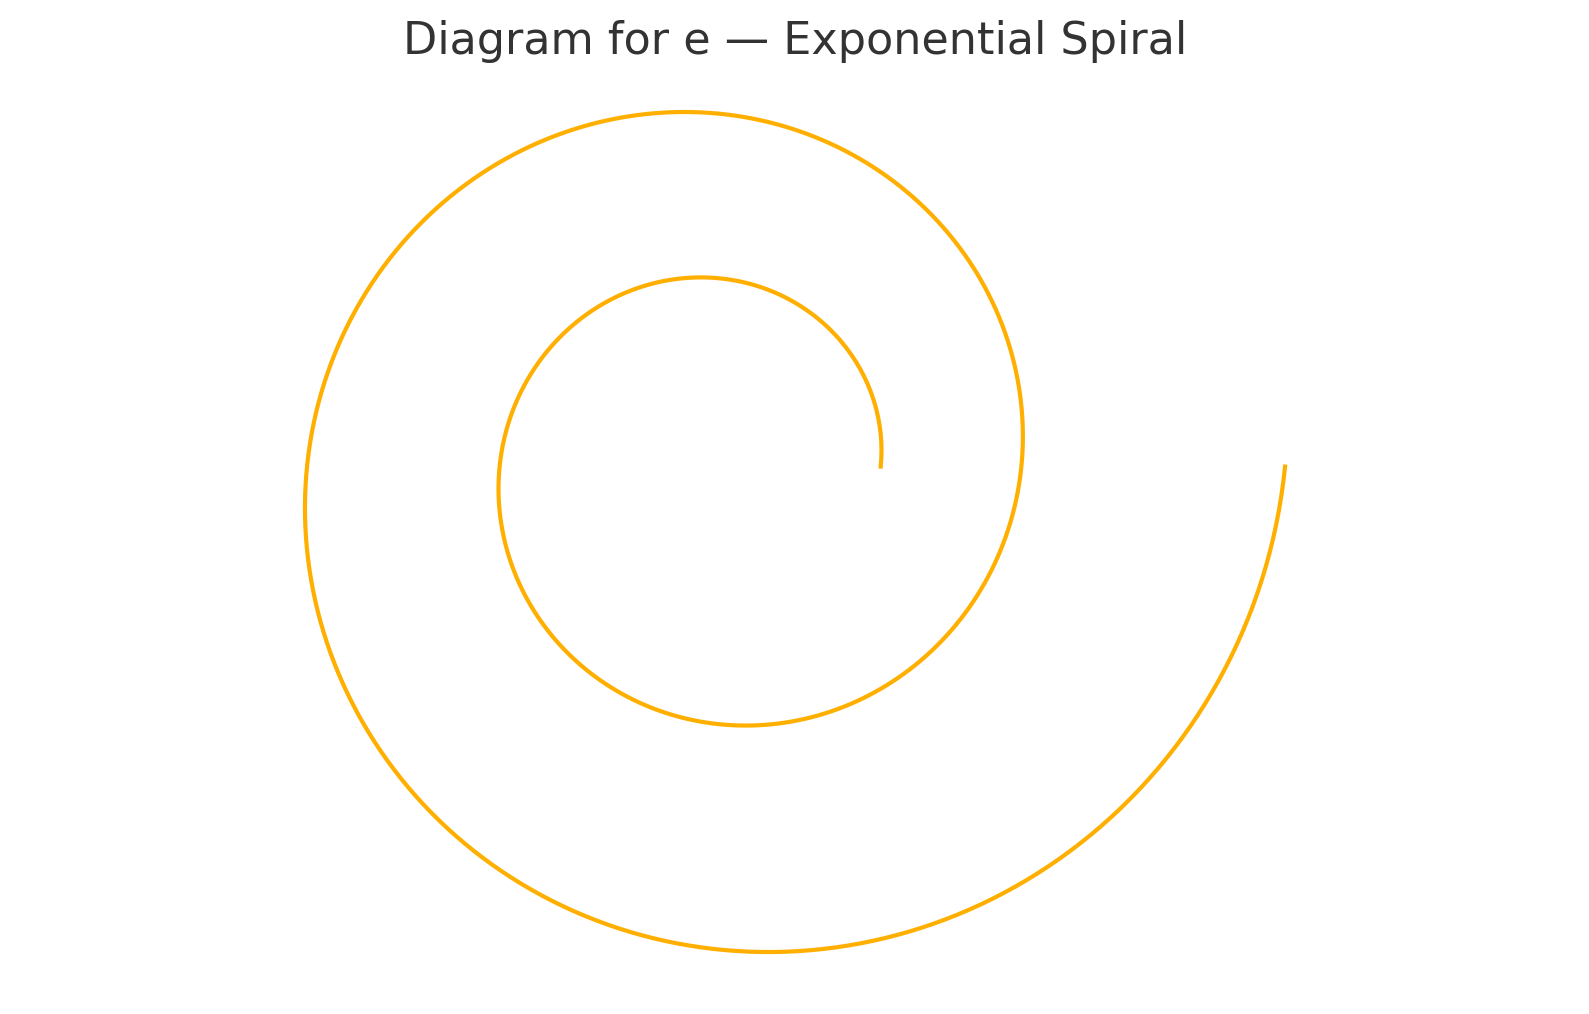
\includegraphics[width=0.4\textwidth]{hs_diagram_e.png}
  \caption{Diagram for $e$ — Exponential Spiral}
\end{figure}

\begin{figure}[h!]
  \centering
  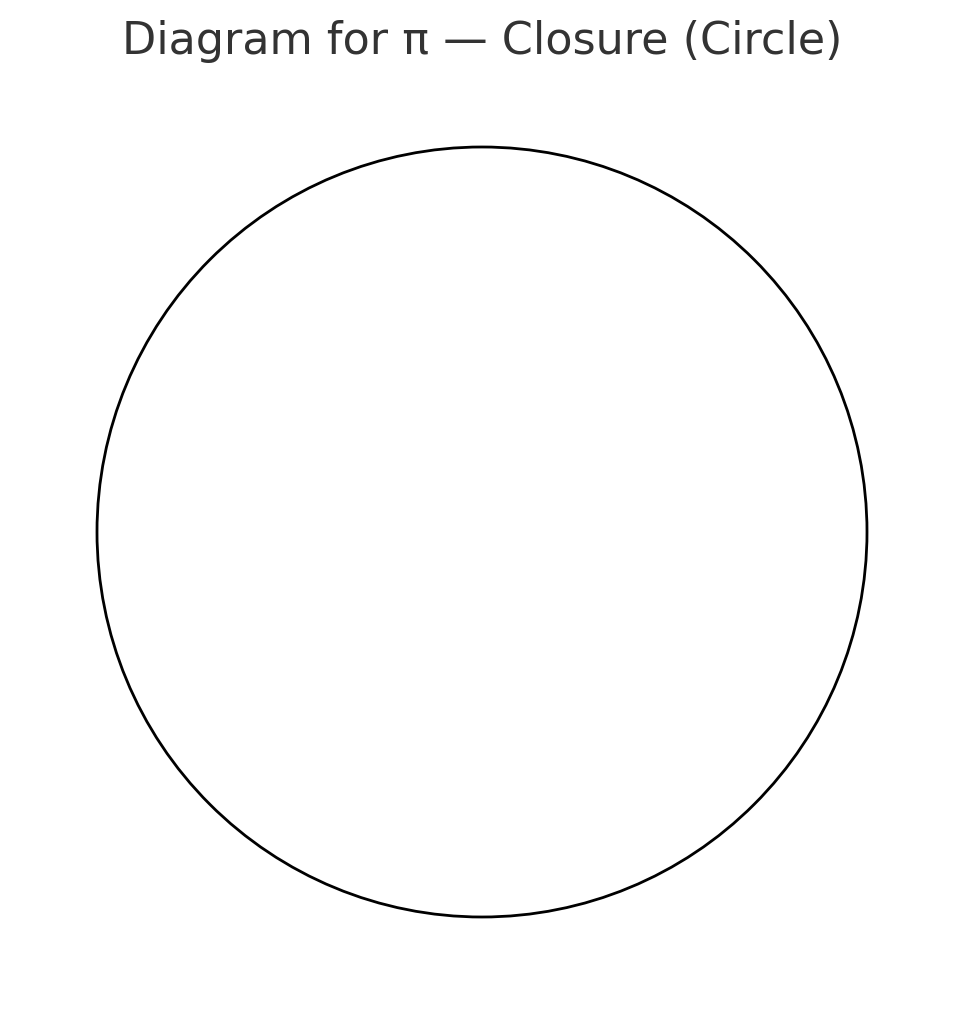
\includegraphics[width=0.4\textwidth]{hs_diagram_pi.png}
  \caption{Diagram for $\pi$ — Closure (Circle)}
\end{figure}

\begin{figure}[h!]
  \centering
  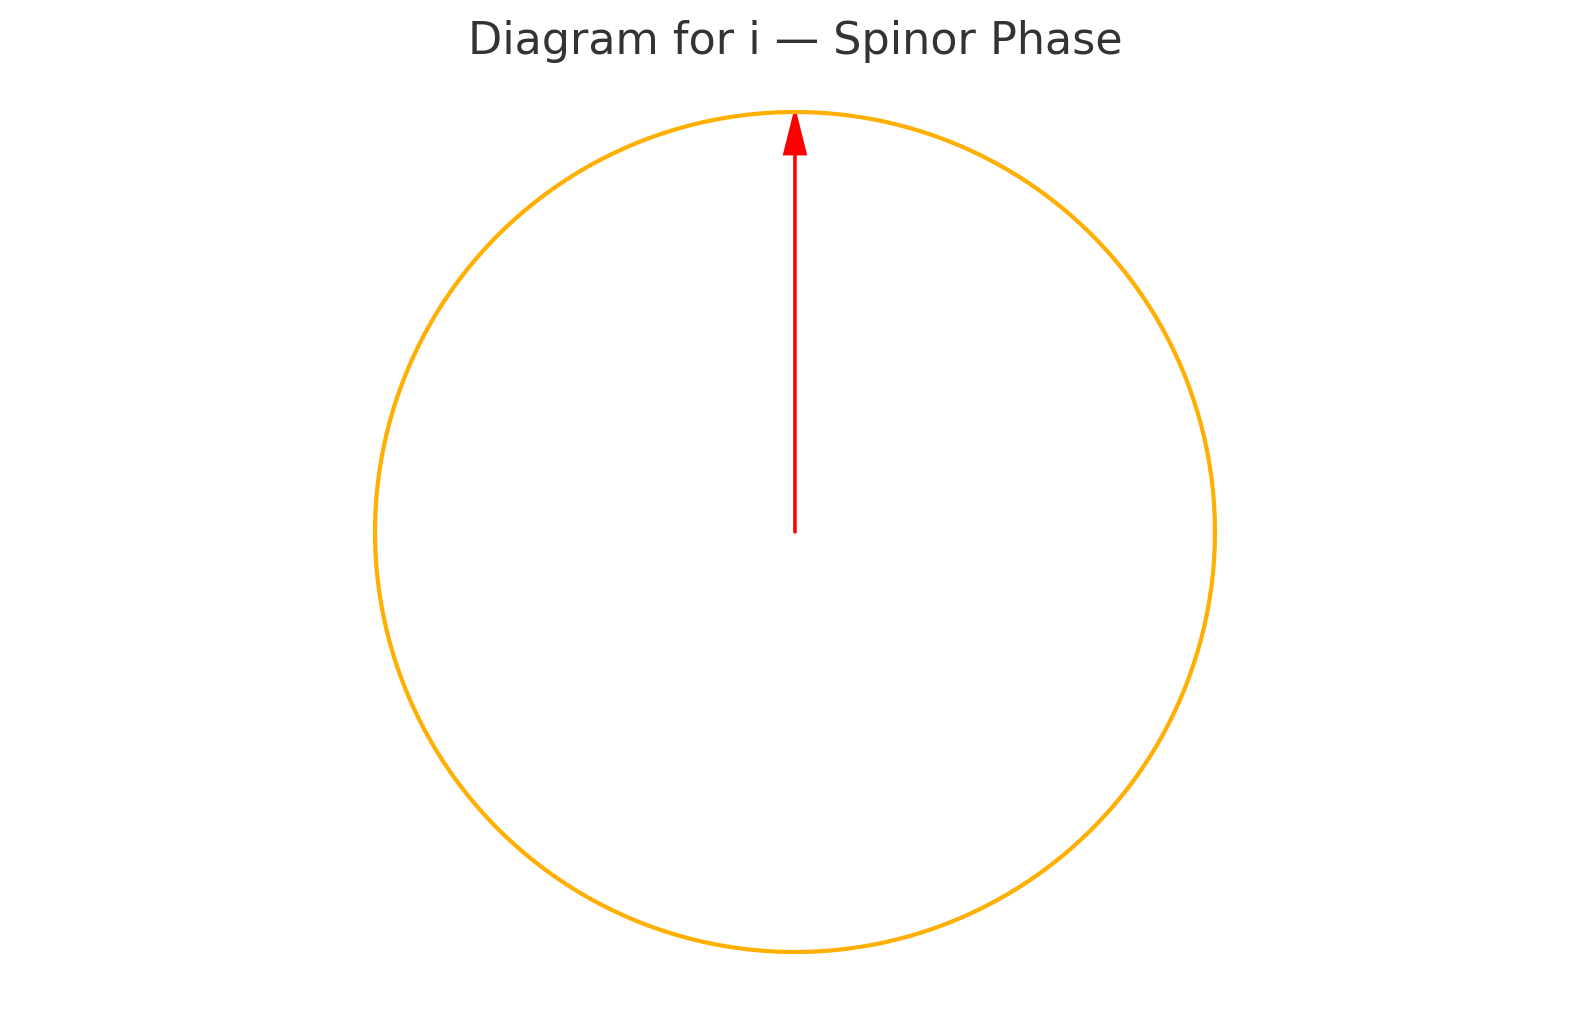
\includegraphics[width=0.4\textwidth]{hs_diagram_i.png}
  \caption{Diagram for $i$ — Spinor Phase}
\end{figure}

\begin{figure}[h!]
  \centering
  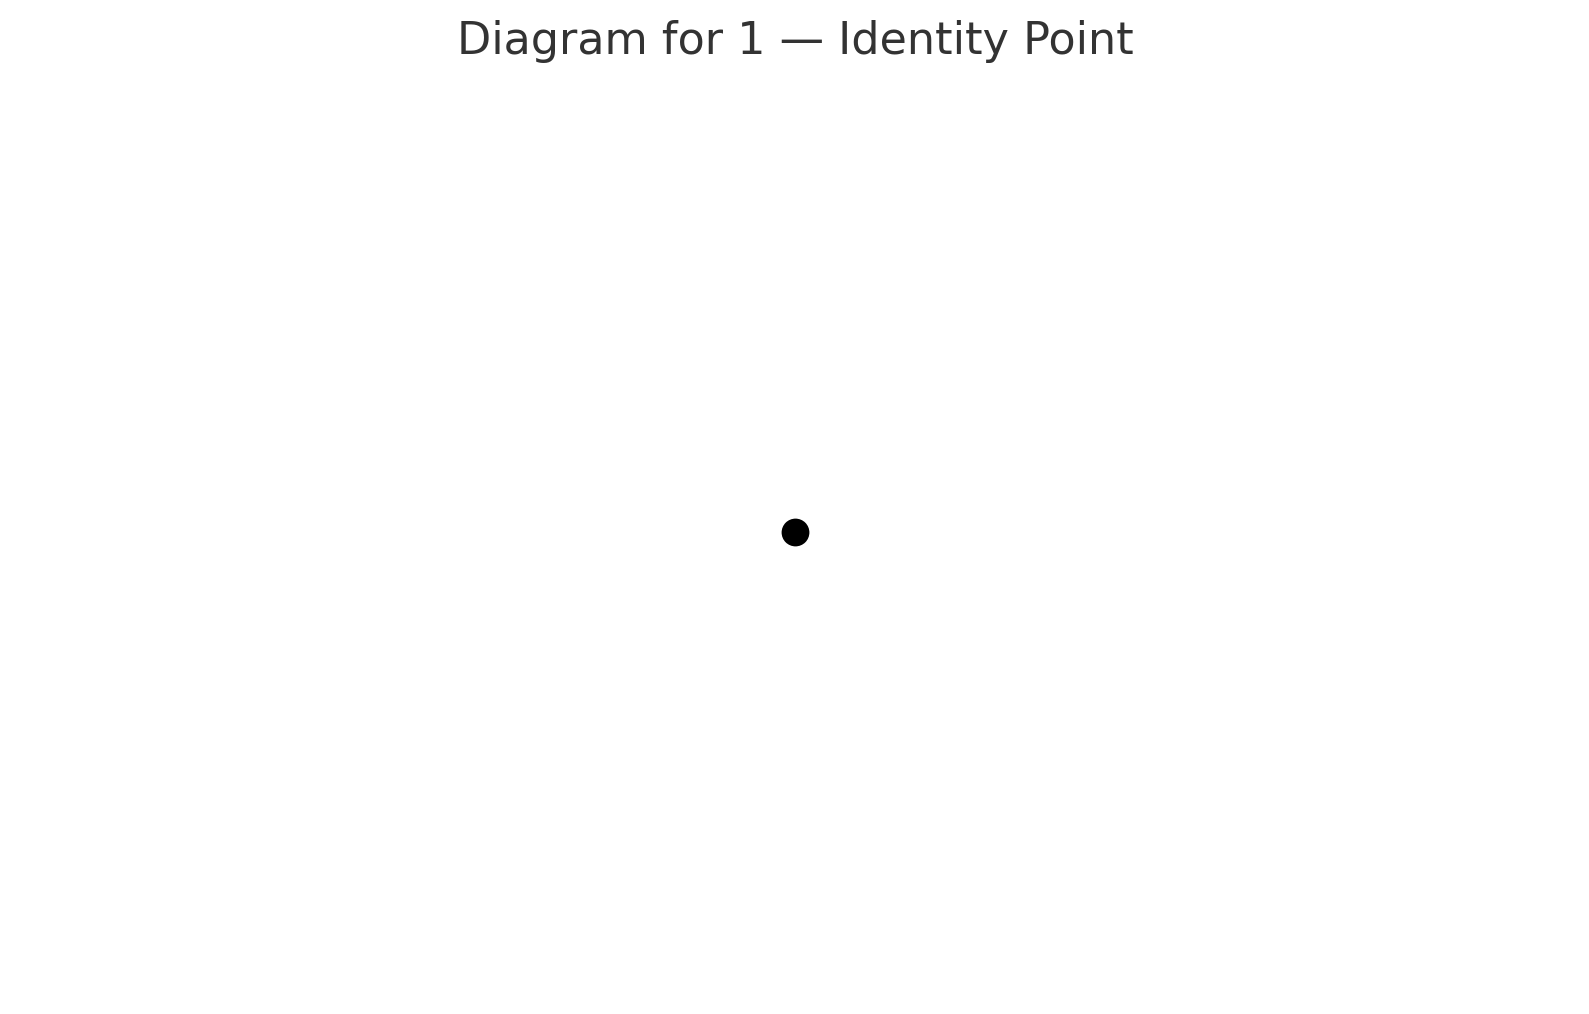
\includegraphics[width=0.2\textwidth]{hs_diagram_1.png}
  \caption{Diagram for $1$ — Identity Point}
\end{figure}

\begin{figure}[h!]
  \centering
  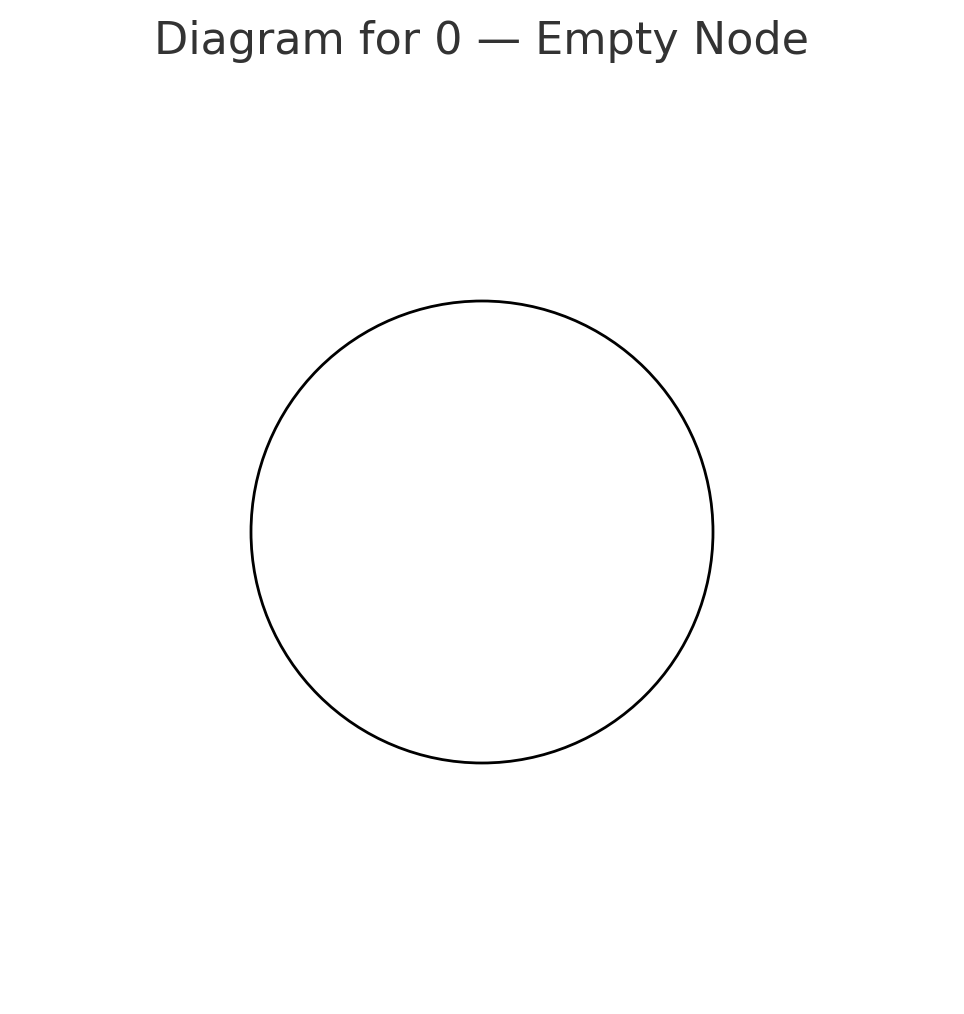
\includegraphics[width=0.2\textwidth]{hs_diagram_0.png}
  \caption{Diagram for $0$ — Empty Node}
\end{figure}

\begin{figure}[h!]
  \centering
  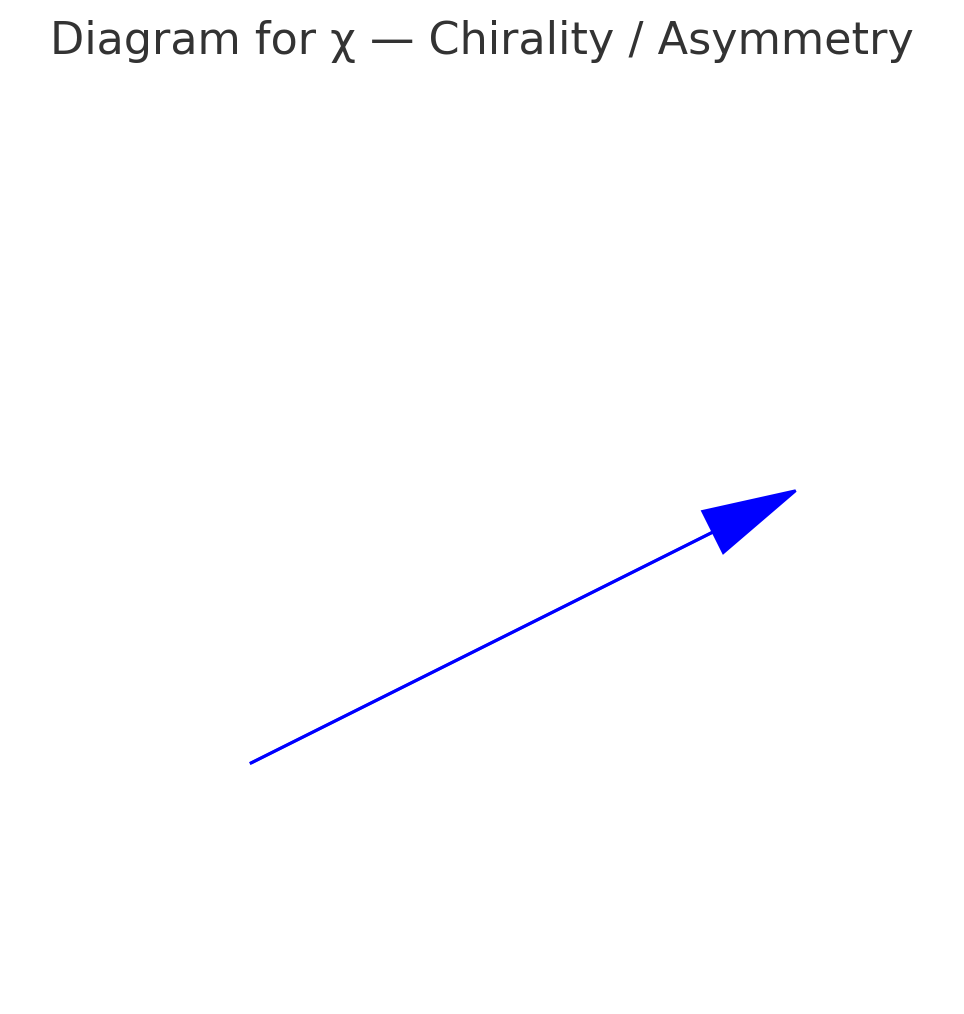
\includegraphics[width=0.4\textwidth]{hs_diagram_chi.png}
  \caption{Diagram for $\chi$ — Chirality / Asymmetry}
\end{figure}
